%%%%%%%%%%%%%%%%%%%%%%%%%%%%%%%%%%%%%%%%%%%%%%%%%%%%%%%%%%%%%%%%%%%%%%%%%%%%%%%%
%%%%%%%%%%%%%%%%%%%%%%%%%%%%%%%%%%%%%%%%%%%%%%%%%%%%%%%%%%%%%%%%%%%%%%%%%%%%%%%%
%%%%%%%%%%%%%%%%%%%%%%%%%%%%%%%%%%%%%%%%%%%%%%%%%%%%%%%%%%%%%%%%%%%%%%%%%%%%%%%%
\section{Notebook et module Python\label{principe-de-largument-de-cauchy}}
%%%%%%%%%%%%%%%%%%%%%%%%%%%%%%%%%%%%%%%%%%%%%%%%%%%%%%%%%%%%%%%%%%%%%%%%%%%%%%%%
%%%%%%%%%%%%%%%%%%%%%%%%%%%%%%%%%%%%%%%%%%%%%%%%%%%%%%%%%%%%%%%%%%%%%%%%%%%%%%%%
%%%%%%%%%%%%%%%%%%%%%%%%%%%%%%%%%%%%%%%%%%%%%%%%%%%%%%%%%%%%%%%%%%%%%%%%%%%%%%%%
Ce notebook permet de tracer l'image d'un contour du plan complexe par
une fonction de transfert quelconque. Le but est de vérifier \textbf{le
principe de l'argument de Cauchy} en partant de cas simples. \textbf{Ce
principe est à la base du critère de Nyquist qui permet d'étudier la
stabilité des systèmes asservis.}
%-------------------------------------------------------------------------------
\begin{center}
\tikzsetnextfilename{nyquist_cauchy-chap_stab-ext}
\begin{tikzpicture}
\begin{axis}
    [
    name=nyy1,
    height=8cm,
    width=8cm,
    axis lines = center,
    ticks=none,
    axis line style = thick,
    enlargelimits=false,
    xlabel=$\Re{p}$,
    ylabel=$\Im{p}$,
    xlabel style={below},
    ylabel style={left},
    ymin=-4,
    ymax=4,
    xmin=-8,
    xmax=8
    ]     
    \pgfmathsetseed{3}
    \draw[
        decoration={markings,mark=at position 0.2 with 
        {\arrow[line width=2pt]{latex}}},
        decoration={markings,mark=at position 0.6 with 
        {\arrow[line width=2pt]{latex}}},
           postaction={decorate},
           thick,
           col4,
           smooth cycle,
           samples=11,
           domain={11:1},
           xshift=3cm,
           yshift=3cm] plot (\x*360/11+5*rnd:1.25cm+0.75cm*rnd) ;
    \node[col4] (ct) at (axis cs:-4,2) {\Large$\mathcal{C}$};
    \addplot[mark=x,ultra thick,only marks,mark size=5pt] 
    coordinates{ (-3.0,-0.5) (-6,-1)};
    \addplot[mark=o,ultra thick,only marks,mark size=5pt] 
    coordinates{ (1,0) (-1,1.2) (-2.1,-1.7) };
\end{axis}
\begin{axis}
    [
    at={(nyy1.south east)},xshift=4ex,
    height=8cm,
    width=8cm,
    axis lines = center,
    ticks=none,
    axis line style = thick,
    enlargelimits=false,
    xlabel=$\Re{F(p)}$,
    ylabel=$\Im{F(p)}$,
    xlabel style={below},
    ylabel style={left},
    ymin=-4,
    ymax=4,
    xmin=-4,
    xmax=4
    ]     
    \def\m{1.0}
    \def\n{2.1}
    \addplot[
    decoration={markings,mark=at position 0.1 with 
    {\arrowreversed[line width=2pt]{latex}}},
    decoration={markings,mark=at position 0.5 with 
    {\arrowreversed[line width=2pt]{latex}}},
    postaction={decorate},
    col1,
    thick,
    domain=1:3,
    samples=50,
    smooth cycle] coordinates 
    {(1.9,-1.5) (0,-2) (-0.75,0.35) (0.25,1.25) (1,0.25) (-0.25,-0.75) 
    (-1.1,-1.25) (-1.5,-1) (-2,0) (-1.5,1.5)  (0,2)  (0.75,1.9) (2,0)}; 
    \node[col1] (ct) at (axis cs:-2.5,2) {\Large$\Gamma:F(\mathcal{C})$};
    \draw[draw=none,fill=black] (axis cs:0,0) circle[radius=2pt];
\end{axis}
\end{tikzpicture}

\end{center}
%-------------------------------------------------------------------------------
Le module qui s'occupe explicitement de calculer et tracer les contours
d'origine et image se trouve dans le fichier \texttt{cauchy\_main.py}.
Ici nous allons simplement importer les fonctions les plus importantes
et apprendre à les manipuler.
L'importation du module se fait par l'instruction suivante:
%-------------------------------------------------------------------------------
\begin{tcolorbox}[breakable, size=fbox, boxrule=1pt, pad at break*=1mm,colback=cellbackground, colframe=cellborder]
\prompt{In}{incolor}{1}{\boxspacing}
\begin{Verbatim}[commandchars=\\\{\}]
\PY{k+kn}{from} \PY{n+nn}{ftransfert} \PY{k}{import} \PY{n}{Ftransfert}
\end{Verbatim}
\end{tcolorbox}
%-------------------------------------------------------------------------------

    La classe \texttt{Ftransfert} permet de définir une fonction de
transfert. Celle-ci sera simplement définie par son gain \(k\), ses
pôles \(p_i\) et ses zéros \(z_i\).

\[
F(p)=k\dfrac{(p-z_1)(p-z_2)(p-z_3)\ldots}{(p-p_1)(p-p_2)(p-p_3)\ldots}
\]

La définition d'une fonction de transfert se fait par l'instuction
suivante:

%-------------------------------------------------------------------------------
\begin{Shaded}
\begin{Highlighting}[]
\NormalTok{zeros}\OperatorTok{=}\NormalTok{[(}\DecValTok{1}\NormalTok{,}\DecValTok{0}\NormalTok{)]  }
\NormalTok{poles}\OperatorTok{=}\NormalTok{[(}\OperatorTok{-}\DecValTok{1}\NormalTok{,}\DecValTok{0}\NormalTok{),(}\OperatorTok{-}\DecValTok{2}\NormalTok{,}\DecValTok{0}\NormalTok{)]}
\NormalTok{gain}\OperatorTok{=}\FloatTok{0.25}
\NormalTok{F}\OperatorTok{=}\NormalTok{Ftransfert(zeros}\OperatorTok{=}\NormalTok{zeros,poles}\OperatorTok{=}\NormalTok{poles,gain}\OperatorTok{=}\NormalTok{gain)}
\end{Highlighting}
\end{Shaded}
%-------------------------------------------------------------------------------

où \texttt{zeros} et \texttt{poles} sont des listes de nombre complexe.
Un segment de points est une liste de nombres complexes modélisés par un
tuple de deux éléments \texttt{(réel,imaginaire)}.

%-------------------------------------------------------------------------------
\begin{tcolorbox}[breakable, size=fbox, boxrule=1pt, pad at break*=1mm,colback=cellbackground, colframe=cellborder]
\prompt{In}{incolor}{2}{\boxspacing}
\begin{Verbatim}[commandchars=\\\{\}]
\PY{n}{zeros}\PY{o}{=}\PY{p}{[}\PY{p}{]}  
\PY{n}{poles}\PY{o}{=}\PY{p}{[}\PY{p}{(}\PY{o}{\PYZhy{}}\PY{l+m+mi}{1}\PY{p}{,}\PY{l+m+mi}{0}\PY{p}{)}\PY{p}{,}\PY{p}{(}\PY{o}{\PYZhy{}}\PY{l+m+mi}{2}\PY{p}{,}\PY{l+m+mi}{0}\PY{p}{)}\PY{p}{]}
\PY{n}{gain}\PY{o}{=}\PY{l+m+mi}{6}
\PY{n}{F}\PY{o}{=}\PY{n}{Ftransfert}\PY{p}{(}\PY{n}{zeros}\PY{o}{=}\PY{n}{zeros}\PY{p}{,}\PY{n}{poles}\PY{o}{=}\PY{n}{poles}\PY{p}{,}\PY{n}{gain}\PY{o}{=}\PY{n}{gain}\PY{p}{)}
\PY{n+nb}{print}\PY{p}{(}\PY{n+nb}{repr}\PY{p}{(}\PY{n}{F}\PY{p}{)}\PY{p}{)}
\PY{n+nb}{print}\PY{p}{(}\PY{n+nb}{str}\PY{p}{(}\PY{n}{F}\PY{p}{)}\PY{p}{)}
\end{Verbatim}
\end{tcolorbox}
%-------------------------------------------------------------------------------

    \begin{Verbatim}[commandchars=\\\{\}]
Ftranfert(zeros=[],poles=[(-1, 0), (-2, 0)],gain=6,name="F")

            6
F(p) = ----------
       (p+1)(p+2)

    \end{Verbatim}

    Pour tracer le diagramme de Nyquist on utilisera la méthode suivante :

%-------------------------------------------------------------------------------
    \begin{tcolorbox}[breakable, size=fbox, boxrule=1pt, pad at break*=1mm,colback=cellbackground, colframe=cellborder]
\prompt{In}{incolor}{3}{\boxspacing}
\begin{Verbatim}[commandchars=\\\{\}]
\PY{k+kn}{import} \PY{n+nn}{matplotlib}\PY{n+nn}{.}\PY{n+nn}{pyplot} \PY{k}{as} \PY{n+nn}{plt} 
\PY{n}{F}\PY{o}{.}\PY{n}{nyquist}\PY{p}{(}\PY{n}{labels}\PY{o}{=}\PY{l+s+sa}{r}\PY{l+s+s2}{\PYZdq{}}\PY{l+s+s2}{\PYZdl{}F(p)\PYZdl{}}\PY{l+s+s2}{\PYZdq{}}\PY{p}{,}\PY{n}{xlim}\PY{o}{=}\PY{p}{(}\PY{o}{\PYZhy{}}\PY{l+m+mi}{2}\PY{p}{,}\PY{l+m+mi}{4}\PY{p}{)}\PY{p}{,}\PY{n}{ylim}\PY{o}{=}\PY{p}{(}\PY{o}{\PYZhy{}}\PY{l+m+mf}{2.5}\PY{p}{,}\PY{l+m+mf}{2.5}\PY{p}{)}\PY{p}{,}\PY{n}{n}\PY{o}{=}\PY{l+m+mi}{4096}\PY{p}{,}\PY{n}{dw}\PY{o}{=}\PY{l+m+mf}{0.01}\PY{p}{)}
\end{Verbatim}
\end{tcolorbox}
%-------------------------------------------------------------------------------

    \begin{Verbatim}[commandchars=\\\{\}]
************************************************************
Nyquist plot : F(p)
Pulsation pas : 0.01
Interval des pulsations -20.48 20.48
Nombre de points 4096

            6
F(p) = ----------
       (p+1)(p+2)

************************************************************
\end{Verbatim}
%-------------------------------------------------------------------------------
\begin{center}
    \includegraphics[width=0.7\textwidth]{notebook/fig/output_5_1.eps}
\end{center}
%-------------------------------------------------------------------------------
%%%%%%%%%%%%%%%%%%%%%%%%%%%%%%%%%%%%%%%%%%%%%%%%%%%%%%%%%%%%%%%%%%%%%%%%%%%%%%%%
%%%%%%%%%%%%%%%%%%%%%%%%%%%%%%%%%%%%%%%%%%%%%%%%%%%%%%%%%%%%%%%%%%%%%%%%%%%%%%%%
%%%%%%%%%%%%%%%%%%%%%%%%%%%%%%%%%%%%%%%%%%%%%%%%%%%%%%%%%%%%%%%%%%%%%%%%%%%%%%%%
\section{Contour dans le plan complexe\label{contour-dans-le-plan-complexe}}
%%%%%%%%%%%%%%%%%%%%%%%%%%%%%%%%%%%%%%%%%%%%%%%%%%%%%%%%%%%%%%%%%%%%%%%%%%%%%%%%
%%%%%%%%%%%%%%%%%%%%%%%%%%%%%%%%%%%%%%%%%%%%%%%%%%%%%%%%%%%%%%%%%%%%%%%%%%%%%%%%
%%%%%%%%%%%%%%%%%%%%%%%%%%%%%%%%%%%%%%%%%%%%%%%%%%%%%%%%%%%%%%%%%%%%%%%%%%%%%%%%
Le module est accompagné de quelques fonctions pour tracer des figures
de contour simple.
%-------------------------------------------------------------------------------
\begin{tcolorbox}[breakable, size=fbox, boxrule=1pt, pad at break*=1mm,colback=cellbackground, colframe=cellborder]
\prompt{In}{incolor}{4}{\boxspacing}
\begin{Verbatim}[commandchars=\\\{\}]
\PY{k+kn}{from} \PY{n+nn}{contour} \PY{k}{import} \PY{n}{rectangle}\PY{p}{,}\PY{n}{circle}\PY{p}{,}\PY{n}{plot\PYZus{}contour}
\end{Verbatim}
\end{tcolorbox}

Commençons par définir un contour de la forme d'un rectangle en
définissant deux coins de coordonnées \texttt{A=(-1.5,-1)} et
\texttt{B=(-0.5,1)} à l'aide de la fonction rectangle. Celle-ci retourne
une liste de quatre liste Python de 64 points chacuns (valeur par
défaut: 128).
On peut également définir le même contour mais parcouru dans le sens
contraire (ici le sens trigonométrique). Nous nommerons ce contour
\texttt{C1\_inv}

    \begin{tcolorbox}[breakable, size=fbox, boxrule=1pt, pad at break*=1mm,colback=cellbackground, colframe=cellborder]
\prompt{In}{incolor}{5}{\boxspacing}
\begin{Verbatim}[commandchars=\\\{\}]
\PY{n}{C1}\PY{o}{=}\PY{n}{rectangle}\PY{p}{(}\PY{p}{(}\PY{l+m+mi}{1}\PY{p}{,}\PY{o}{\PYZhy{}}\PY{l+m+mi}{1}\PY{p}{)}\PY{p}{,}\PY{p}{(}\PY{l+m+mi}{2}\PY{p}{,}\PY{l+m+mi}{1}\PY{p}{)}\PY{p}{,}\PY{n}{npts}\PY{o}{=}\PY{l+m+mi}{64}\PY{p}{)}
\PY{n}{plot\PYZus{}contour}\PY{p}{(}\PY{n}{C1}\PY{p}{,}\PY{n}{xlim}\PY{o}{=}\PY{p}{(}\PY{o}{\PYZhy{}}\PY{l+m+mi}{2}\PY{p}{,}\PY{l+m+mf}{3.5}\PY{p}{)}\PY{p}{,}\PY{n}{ylim}\PY{o}{=}\PY{p}{(}\PY{o}{\PYZhy{}}\PY{l+m+mf}{1.5}\PY{p}{,}\PY{l+m+mf}{1.5}\PY{p}{)}\PY{p}{)}
\PY{n}{C1\PYZus{}inv}\PY{o}{=}\PY{n}{rectangle}\PY{p}{(}\PY{p}{(}\PY{l+m+mi}{1}\PY{p}{,}\PY{o}{\PYZhy{}}\PY{l+m+mi}{1}\PY{p}{)}\PY{p}{,}\PY{p}{(}\PY{l+m+mi}{2}\PY{p}{,}\PY{l+m+mi}{1}\PY{p}{)}\PY{p}{,}\PY{n}{npts}\PY{o}{=}\PY{l+m+mi}{64}\PY{p}{,}\PY{n}{inverse}\PY{o}{=}\PY{k+kc}{True}\PY{p}{)}
\PY{n}{plot\PYZus{}contour}\PY{p}{(}\PY{n}{C1\PYZus{}inv}\PY{p}{,}\PY{n}{xlim}\PY{o}{=}\PY{p}{(}\PY{o}{\PYZhy{}}\PY{l+m+mi}{2}\PY{p}{,}\PY{l+m+mf}{3.5}\PY{p}{)}\PY{p}{,}\PY{n}{ylim}\PY{o}{=}\PY{p}{(}\PY{o}{\PYZhy{}}\PY{l+m+mf}{1.5}\PY{p}{,}\PY{l+m+mf}{1.5}\PY{p}{)}\PY{p}{)}
\end{Verbatim}
\end{tcolorbox}
%-------------------------------------------------------------------------------
%-------------------------------------------------------------------------------
\begin{center}
    \includegraphics[width=0.45\textwidth]{notebook/fig/output_9_0.eps}
    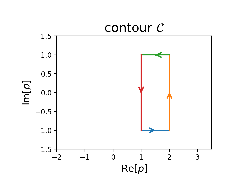
\includegraphics[width=0.45\textwidth]{notebook/fig/output_11_0.eps}
\end{center}
%-------------------------------------------------------------------------------
%%%%%%%%%%%%%%%%%%%%%%%%%%%%%%%%%%%%%%%%%%%%%%%%%%%%%%%%%%%%%%%%%%%%%%%%%%%%%%%%
%%%%%%%%%%%%%%%%%%%%%%%%%%%%%%%%%%%%%%%%%%%%%%%%%%%%%%%%%%%%%%%%%%%%%%%%%%%%%%%%
%%%%%%%%%%%%%%%%%%%%%%%%%%%%%%%%%%%%%%%%%%%%%%%%%%%%%%%%%%%%%%%%%%%%%%%%%%%%%%%%
\section{Image d'un contour par une fonction de transfert
\label{image-dun-contour-par-une-fonction-de-transfert}}
%%%%%%%%%%%%%%%%%%%%%%%%%%%%%%%%%%%%%%%%%%%%%%%%%%%%%%%%%%%%%%%%%%%%%%%%%%%%%%%%
%%%%%%%%%%%%%%%%%%%%%%%%%%%%%%%%%%%%%%%%%%%%%%%%%%%%%%%%%%%%%%%%%%%%%%%%%%%%%%%%
%%%%%%%%%%%%%%%%%%%%%%%%%%%%%%%%%%%%%%%%%%%%%%%%%%%%%%%%%%%%%%%%%%%%%%%%%%%%%%%%
%%%%%%%%%%%%%%%%%%%%%%%%%%%%%%%%%%%%%%%%%%%%%%%%%%%%%%%%%%%%%%%%%%%%%%%%%%%%%%%%
%%%%%%%%%%%%%%%%%%%%%%%%%%%%%%%%%%%%%%%%%%%%%%%%%%%%%%%%%%%%%%%%%%%%%%%%%%%%%%%%
\subsection{Fonction de transfert avec un seul zéro
\label{fonction-de-transfert-avec-un-seul-zuxe9ro}}
%%%%%%%%%%%%%%%%%%%%%%%%%%%%%%%%%%%%%%%%%%%%%%%%%%%%%%%%%%%%%%%%%%%%%%%%%%%%%%%%
%%%%%%%%%%%%%%%%%%%%%%%%%%%%%%%%%%%%%%%%%%%%%%%%%%%%%%%%%%%%%%%%%%%%%%%%%%%%%%%%
Déterminons maintenant l'image de ces contours par une fonction de
transfert composée d'un seul zéro (\(z_1=-1\)).
\[
F_1(p)=(p+1)
\]
%-------------------------------------------------------------------------------
\begin{tcolorbox}[breakable, size=fbox, boxrule=1pt, pad at break*=1mm,colback=cellbackground, colframe=cellborder]
\prompt{In}{incolor}{7}{\boxspacing}
\begin{Verbatim}[commandchars=\\\{\}]
\PY{n}{poles}\PY{o}{=}\PY{p}{[}\PY{p}{]}
\PY{n}{zeros}\PY{o}{=}\PY{p}{[}\PY{p}{(}\PY{o}{\PYZhy{}}\PY{l+m+mi}{1}\PY{p}{,}\PY{l+m+mi}{0}\PY{p}{)}\PY{p}{]}
\PY{n}{gain}\PY{o}{=}\PY{l+m+mi}{1}
\PY{n}{F\PYZus{}1}\PY{o}{=}\PY{n}{Ftransfert}\PY{p}{(}\PY{n}{zeros}\PY{o}{=}\PY{n}{zeros}\PY{p}{,}\PY{n}{poles}\PY{o}{=}\PY{n}{poles}\PY{p}{,}\PY{n}{gain}\PY{o}{=}\PY{n}{gain}\PY{p}{,}\PY{n}{name}\PY{o}{=}\PY{l+s+s2}{\PYZdq{}}\PY{l+s+s2}{F\PYZus{}1}\PY{l+s+s2}{\PYZdq{}}\PY{p}{)}
\end{Verbatim}
\end{tcolorbox}
%-------------------------------------------------------------------------------
%%%%%%%%%%%%%%%%%%%%%%%%%%%%%%%%%%%%%%%%%%%%%%%%%%%%%%%%%%%%%%%%%%%%%%%%%%%%%%%%
\subsubsection{Contour ne contenant pas le zéro parcouru\label{contour-nentourant-pas-le-zuxe9ro-parcouru}}
%%%%%%%%%%%%%%%%%%%%%%%%%%%%%%%%%%%%%%%%%%%%%%%%%%%%%%%%%%%%%%%%%%%%%%%%%%%%%%%%
%%%%%%%%%%%%%%%%%%%%%%%%%%%%%%%%%%%%%%%%%%%%%%%%%%%%%%%%%%%%%%%%%%%%%%%%%%%%%%%%
\paragraph{\ldots{} dans le sens horaire\label{dans-le-sens-horaire}}
%%%%%%%%%%%%%%%%%%%%%%%%%%%%%%%%%%%%%%%%%%%%%%%%%%%%%%%%%%%%%%%%%%%%%%%%%%%%%%%%
%-------------------------------------------------------------------------------
\begin{tcolorbox}[breakable, size=fbox, boxrule=1pt, pad at break*=1mm,colback=cellbackground, colframe=cellborder]
\prompt{In}{incolor}{8}{\boxspacing}
\begin{Verbatim}[commandchars=\\\{\}]
\PY{n}{F\PYZus{}1}\PY{o}{.}\PY{n}{cauchy}\PY{p}{(}\PY{n}{C1}\PY{p}{,}\PY{n}{xlim}\PY{o}{=}\PY{p}{(}\PY{o}{\PYZhy{}}\PY{l+m+mi}{2}\PY{p}{,}\PY{l+m+mf}{3.5}\PY{p}{)}\PY{p}{,}\PY{n}{ylim}\PY{o}{=}\PY{p}{(}\PY{o}{\PYZhy{}}\PY{l+m+mf}{1.5}\PY{p}{,}\PY{l+m+mf}{1.5}\PY{p}{)}\PY{p}{,}\PY{n}{contourLabel}\PY{o}{=}\PY{l+s+s2}{\PYZdq{}}\PY{l+s+s2}{C1}\PY{l+s+s2}{\PYZdq{}}\PY{p}{)}
\end{Verbatim}
\end{tcolorbox}
%-------------------------------------------------------------------------------
%-------------------------------------------------------------------------------
\begin{center}
    \includegraphics[width=0.9\textwidth]{notebook/fig/output_15_1.eps}
\end{center}
%-------------------------------------------------------------------------------
%%%%%%%%%%%%%%%%%%%%%%%%%%%%%%%%%%%%%%%%%%%%%%%%%%%%%%%%%%%%%%%%%%%%%%%%%%%%%%%%
\paragraph{\ldots{} Dans le sens trigonométrique\label{dans-le-sens-trigonomuxe9trique}}
%%%%%%%%%%%%%%%%%%%%%%%%%%%%%%%%%%%%%%%%%%%%%%%%%%%%%%%%%%%%%%%%%%%%%%%%%%%%%%%%
%-------------------------------------------------------------------------------
\begin{tcolorbox}[breakable, size=fbox, boxrule=1pt, pad at break*=1mm,colback=cellbackground, colframe=cellborder]
\prompt{In}{incolor}{9}{\boxspacing}
\begin{Verbatim}[commandchars=\\\{\}]
\PY{n}{F\PYZus{}1}\PY{o}{.}\PY{n}{cauchy}\PY{p}{(}\PY{n}{C1\PYZus{}inv}\PY{p}{,}\PY{n}{xlim}\PY{o}{=}\PY{p}{(}\PY{o}{\PYZhy{}}\PY{l+m+mi}{2}\PY{p}{,}\PY{l+m+mf}{3.5}\PY{p}{)}\PY{p}{,}\PY{n}{ylim}\PY{o}{=}\PY{p}{(}\PY{o}{\PYZhy{}}\PY{l+m+mf}{1.5}\PY{p}{,}\PY{l+m+mf}{1.5}\PY{p}{)}\PY{p}{,}\PY{n}{contourLabel}\PY{o}{=}\PY{l+s+s2}{\PYZdq{}}\PY{l+s+s2}{C1 (inverse)}\PY{l+s+s2}{\PYZdq{}}\PY{p}{)}
\end{Verbatim}
\end{tcolorbox}
%-------------------------------------------------------------------------------
%-------------------------------------------------------------------------------
\begin{center}
    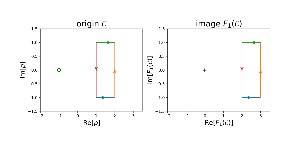
\includegraphics[width=0.9\textwidth]{notebook/fig/output_17_1.eps}
\end{center}
%-------------------------------------------------------------------------------
(La carte des pôles et zéros de la fonction de transfert sera toujours
représentée sur le graphe de gauche. Sur le graphe de droite c'est
l'origine du plan qui sera toujours représentée par un `+'.)
Nous constatons que l'image du contour par une telle fonction de
transfert est simplement translatée d'une distance égale à la distance
entre le point du contour et la position du zéro. \textbf{Nous observons
également que le sens de parcours du contour de l'image n'est pas
modifié.}
%%%%%%%%%%%%%%%%%%%%%%%%%%%%%%%%%%%%%%%%%%%%%%%%%%%%%%%%%%%%%%%%%%%%%%%%%%%%%%%%
\subsubsection{Contour contenant le zéro\label{contour-contenant-le-zuxe9ro}}
%%%%%%%%%%%%%%%%%%%%%%%%%%%%%%%%%%%%%%%%%%%%%%%%%%%%%%%%%%%%%%%%%%%%%%%%%%%%%%%%
On se donne un deuxième contour \texttt{C2} qui contient le zéro de la
fonction de transfert test.
%-------------------------------------------------------------------------------
\begin{tcolorbox}[breakable, size=fbox, boxrule=1pt, pad at break*=1mm,colback=cellbackground, colframe=cellborder]
\prompt{In}{incolor}{10}{\boxspacing}
\begin{Verbatim}[commandchars=\\\{\}]
\PY{n}{C2}\PY{o}{=}\PY{n}{rectangle}\PY{p}{(}\PY{p}{(}\PY{o}{\PYZhy{}}\PY{l+m+mf}{1.5}\PY{p}{,}\PY{o}{\PYZhy{}}\PY{l+m+mi}{1}\PY{p}{)}\PY{p}{,}\PY{p}{(}\PY{o}{\PYZhy{}}\PY{l+m+mf}{0.5}\PY{p}{,}\PY{l+m+mi}{1}\PY{p}{)}\PY{p}{,}\PY{n}{npts}\PY{o}{=}\PY{l+m+mi}{64}\PY{p}{)}
\PY{n}{C2\PYZus{}inv}\PY{o}{=}\PY{n}{rectangle}\PY{p}{(}\PY{p}{(}\PY{o}{\PYZhy{}}\PY{l+m+mf}{1.5}\PY{p}{,}\PY{o}{\PYZhy{}}\PY{l+m+mi}{1}\PY{p}{)}\PY{p}{,}\PY{p}{(}\PY{o}{\PYZhy{}}\PY{l+m+mf}{0.5}\PY{p}{,}\PY{l+m+mi}{1}\PY{p}{)}\PY{p}{,}\PY{n}{npts}\PY{o}{=}\PY{l+m+mi}{64}\PY{p}{,}\PY{n}{inverse}\PY{o}{=}\PY{k+kc}{True}\PY{p}{)}
\end{Verbatim}
\end{tcolorbox}
%-------------------------------------------------------------------------------
%-------------------------------------------------------------------------------
\begin{tcolorbox}[breakable, size=fbox, boxrule=1pt, pad at break*=1mm,colback=cellbackground, colframe=cellborder]
\prompt{In}{incolor}{11}{\boxspacing}
\begin{Verbatim}[commandchars=\\\{\}]
\PY{n}{F\PYZus{}1}\PY{o}{.}\PY{n}{cauchy}\PY{p}{(}\PY{n}{C2}\PY{p}{,}\PY{n}{xlim}\PY{o}{=}\PY{p}{(}\PY{o}{\PYZhy{}}\PY{l+m+mi}{2}\PY{p}{,}\PY{l+m+mi}{1}\PY{p}{)}\PY{p}{,}\PY{n}{ylim}\PY{o}{=}\PY{p}{(}\PY{o}{\PYZhy{}}\PY{l+m+mf}{1.5}\PY{p}{,}\PY{l+m+mf}{1.5}\PY{p}{)}\PY{p}{,}\PY{n}{contourLabel}\PY{o}{=}\PY{l+s+s2}{\PYZdq{}}\PY{l+s+s2}{C2}\PY{l+s+s2}{\PYZdq{}}\PY{p}{)}
\end{Verbatim}
\end{tcolorbox}
%-------------------------------------------------------------------------------
%-------------------------------------------------------------------------------
\begin{center}
    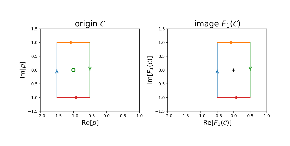
\includegraphics[width=0.9\textwidth]{notebook/fig/output_20_1.eps}
\end{center}
%-------------------------------------------------------------------------------
%-------------------------------------------------------------------------------
\begin{tcolorbox}[breakable, size=fbox, boxrule=1pt, pad at break*=1mm,colback=cellbackground, colframe=cellborder]
\prompt{In}{incolor}{12}{\boxspacing}
\begin{Verbatim}[commandchars=\\\{\}]
\PY{n}{F\PYZus{}1}\PY{o}{.}\PY{n}{cauchy}\PY{p}{(}\PY{n}{C2\PYZus{}inv}\PY{p}{,}\PY{n}{xlim}\PY{o}{=}\PY{p}{(}\PY{o}{\PYZhy{}}\PY{l+m+mi}{2}\PY{p}{,}\PY{l+m+mi}{1}\PY{p}{)}\PY{p}{,}\PY{n}{ylim}\PY{o}{=}\PY{p}{(}\PY{o}{\PYZhy{}}\PY{l+m+mf}{1.5}\PY{p}{,}\PY{l+m+mf}{1.5}\PY{p}{)}\PY{p}{,}\PY{n}{contourLabel}\PY{o}{=}\PY{l+s+s2}{\PYZdq{}}\PY{l+s+s2}{C2 (inverse)}\PY{l+s+s2}{\PYZdq{}}\PY{p}{)}
\end{Verbatim}
\end{tcolorbox}
%-------------------------------------------------------------------------------
%-------------------------------------------------------------------------------
\begin{center}
    \includegraphics[width=0.9\textwidth]{notebook/fig/output_21_1.eps}
\end{center}
%-------------------------------------------------------------------------------
\textbf{Ici le contour \(\mathcal{C}\) entoure le zéro de la fonction de
transfert. Nous observons que le contour image contient l'origine (et
est orienté dans le même sens que le contour origine).} \#\# Fonction de
transfert avec deux zéros
Traçons maintenant le résultat pour une fonction de transfert possédant
deux zéros (\(z_1=-1\) et \(z_2=-0.75\)):
\[
F_2(p)=\dfrac{1}{4}(p+1)(p+0.75).
\]
%%%%%%%%%%%%%%%%%%%%%%%%%%%%%%%%%%%%%%%%%%%%%%%%%%%%%%%%%%%%%%%%%%%%%%%%%%%%%%%%
\subsubsection{Contour ne contenant pas les zéros\label{contour-nentourant-pas-les-zuxe9ros}}
%%%%%%%%%%%%%%%%%%%%%%%%%%%%%%%%%%%%%%%%%%%%%%%%%%%%%%%%%%%%%%%%%%%%%%%%%%%%%%%%
%-------------------------------------------------------------------------------
\begin{tcolorbox}[breakable, size=fbox, boxrule=1pt, pad at break*=1mm,colback=cellbackground, colframe=cellborder]
\prompt{In}{incolor}{13}{\boxspacing}
\begin{Verbatim}[commandchars=\\\{\}]
\PY{n}{zeros}\PY{o}{=}\PY{p}{[}\PY{p}{(}\PY{o}{\PYZhy{}}\PY{l+m+mi}{1}\PY{p}{,}\PY{l+m+mi}{0}\PY{p}{)}\PY{p}{,}\PY{p}{(}\PY{o}{\PYZhy{}}\PY{l+m+mf}{0.75}\PY{p}{,}\PY{l+m+mi}{0}\PY{p}{)}\PY{p}{]}
\PY{n}{poles}\PY{o}{=}\PY{p}{[}\PY{p}{]}
\PY{n}{gain}\PY{o}{=}\PY{l+m+mf}{0.25}
\PY{n}{F\PYZus{}2}\PY{o}{=}\PY{n}{Ftransfert}\PY{p}{(}\PY{n}{zeros}\PY{o}{=}\PY{n}{zeros}\PY{p}{,}\PY{n}{poles}\PY{o}{=}\PY{n}{poles}\PY{p}{,}\PY{n}{gain}\PY{o}{=}\PY{n}{gain}\PY{p}{,}\PY{n}{name}\PY{o}{=}\PY{l+s+s2}{\PYZdq{}}\PY{l+s+s2}{F\PYZus{}2}\PY{l+s+s2}{\PYZdq{}}\PY{p}{)}
\end{Verbatim}
\end{tcolorbox}
%-------------------------------------------------------------------------------
%-------------------------------------------------------------------------------
\begin{tcolorbox}[breakable, size=fbox, boxrule=1pt, pad at break*=1mm,colback=cellbackground, colframe=cellborder]
\prompt{In}{incolor}{14}{\boxspacing}
\begin{Verbatim}[commandchars=\\\{\}]
\PY{n}{F\PYZus{}2}\PY{o}{.}\PY{n}{cauchy}\PY{p}{(}\PY{n}{C1}\PY{p}{,}\PY{n}{xlim}\PY{o}{=}\PY{p}{(}\PY{o}{\PYZhy{}}\PY{l+m+mi}{2}\PY{p}{,}\PY{l+m+mf}{3.5}\PY{p}{)}\PY{p}{,}\PY{n}{ylim}\PY{o}{=}\PY{p}{(}\PY{o}{\PYZhy{}}\PY{l+m+mf}{1.5}\PY{p}{,}\PY{l+m+mf}{1.5}\PY{p}{)}\PY{p}{,}\PY{n}{contourLabel}\PY{o}{=}\PY{l+s+s2}{\PYZdq{}}\PY{l+s+s2}{C1}\PY{l+s+s2}{\PYZdq{}}\PY{p}{)}
\end{Verbatim}
\end{tcolorbox}
%-------------------------------------------------------------------------------
%-------------------------------------------------------------------------------
\begin{center}
    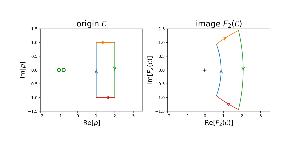
\includegraphics[width=0.9\textwidth]{notebook/fig/output_24_1.eps}
\end{center}
%-------------------------------------------------------------------------------
%-------------------------------------------------------------------------------
\begin{tcolorbox}[breakable, size=fbox, boxrule=1pt, pad at break*=1mm,colback=cellbackground, colframe=cellborder]
\prompt{In}{incolor}{15}{\boxspacing}
\begin{Verbatim}[commandchars=\\\{\}]
\PY{n}{F\PYZus{}2}\PY{o}{.}\PY{n}{cauchy}\PY{p}{(}\PY{n}{C1\PYZus{}inv}\PY{p}{,}\PY{n}{xlim}\PY{o}{=}\PY{p}{(}\PY{o}{\PYZhy{}}\PY{l+m+mi}{2}\PY{p}{,}\PY{l+m+mf}{3.5}\PY{p}{)}\PY{p}{,}\PY{n}{ylim}\PY{o}{=}\PY{p}{(}\PY{o}{\PYZhy{}}\PY{l+m+mf}{1.5}\PY{p}{,}\PY{l+m+mf}{1.5}\PY{p}{)}\PY{p}{,}\PY{n}{contourLabel}\PY{o}{=}\PY{l+s+s2}{\PYZdq{}}\PY{l+s+s2}{C1 (inverse)}\PY{l+s+s2}{\PYZdq{}}\PY{p}{)}
\end{Verbatim}
\end{tcolorbox}
%-------------------------------------------------------------------------------
%-------------------------------------------------------------------------------
\begin{center}
    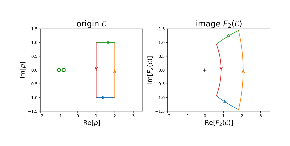
\includegraphics[width=0.9\textwidth]{notebook/fig/output_25_1.eps}
\end{center}
%-------------------------------------------------------------------------------
\textbf{On observe comme précédemment que si le contour ne contient pas
les zéros de la fonction de transfert, l'image de celui-ci ne fait aucun
tour autour de l'origine.} \#\#\# Contour entourant les deux zéros Dans
cet exemple, nous allons utiliser un nouveau contour de la forme d'un
cercle.
%-------------------------------------------------------------------------------
%-------------------------------------------------------------------------------
\begin{tcolorbox}[breakable, size=fbox, boxrule=1pt, pad at break*=1mm,colback=cellbackground, colframe=cellborder]
\prompt{In}{incolor}{16}{\boxspacing}
\begin{Verbatim}[commandchars=\\\{\}]
\PY{n}{C3}\PY{o}{=}\PY{n}{circle}\PY{p}{(}\PY{n}{center}\PY{o}{=}\PY{p}{(}\PY{o}{\PYZhy{}}\PY{l+m+mi}{1}\PY{p}{,}\PY{l+m+mi}{0}\PY{p}{)}\PY{p}{,}\PY{n}{radius}\PY{o}{=}\PY{l+m+mf}{0.75}\PY{p}{)}
\PY{n}{C3\PYZus{}inv}\PY{o}{=}\PY{n}{circle}\PY{p}{(}\PY{n}{center}\PY{o}{=}\PY{p}{(}\PY{o}{\PYZhy{}}\PY{l+m+mi}{1}\PY{p}{,}\PY{l+m+mi}{0}\PY{p}{)}\PY{p}{,}\PY{n}{radius}\PY{o}{=}\PY{l+m+mf}{0.75}\PY{p}{,}\PY{n}{inverse}\PY{o}{=}\PY{k+kc}{True}\PY{p}{)}
\end{Verbatim}
\end{tcolorbox}
%-------------------------------------------------------------------------------
%-------------------------------------------------------------------------------
\begin{tcolorbox}[breakable, size=fbox, boxrule=1pt, pad at break*=1mm,colback=cellbackground, colframe=cellborder]
\prompt{In}{incolor}{17}{\boxspacing}
\begin{Verbatim}[commandchars=\\\{\}]
\PY{n}{F\PYZus{}2}\PY{o}{.}\PY{n}{cauchy}\PY{p}{(}\PY{n}{C3}\PY{p}{,}\PY{n}{xlim}\PY{o}{=}\PY{p}{[}\PY{p}{(}\PY{o}{\PYZhy{}}\PY{l+m+mf}{1.9}\PY{p}{,}\PY{l+m+mf}{1.0}\PY{p}{)}\PY{p}{,}\PY{p}{(}\PY{o}{\PYZhy{}}\PY{l+m+mf}{0.3}\PY{p}{,}\PY{l+m+mf}{0.3}\PY{p}{)}\PY{p}{]}\PY{p}{,}\PY{n}{ylim}\PY{o}{=}\PY{p}{[}\PY{p}{(}\PY{o}{\PYZhy{}}\PY{l+m+mi}{1}\PY{p}{,}\PY{l+m+mi}{1}\PY{p}{)}\PY{p}{,}\PY{p}{(}\PY{o}{\PYZhy{}}\PY{l+m+mf}{0.25}\PY{p}{,}\PY{l+m+mf}{0.25}\PY{p}{)}\PY{p}{]}\PY{p}{,}\PY{n}{contourLabel}\PY{o}{=}\PY{l+s+s2}{\PYZdq{}}\PY{l+s+s2}{C1}\PY{l+s+s2}{\PYZdq{}}\PY{p}{)}
\end{Verbatim}
\end{tcolorbox}
%-------------------------------------------------------------------------------
%-------------------------------------------------------------------------------
\begin{center}
    
\includegraphics[width=0.9\textwidth]{notebook/fig/output_28_1.eps}
\end{center}
%-------------------------------------------------------------------------------
%-------------------------------------------------------------------------------
\begin{tcolorbox}[breakable, size=fbox, boxrule=1pt, pad at break*=1mm,colback=cellbackground, colframe=cellborder]
\prompt{In}{incolor}{18}{\boxspacing}
\begin{Verbatim}[commandchars=\\\{\}]
\PY{n}{F\PYZus{}2}\PY{o}{.}\PY{n}{cauchy}\PY{p}{(}\PY{n}{C3\PYZus{}inv}\PY{p}{,}\PY{n}{xlim}\PY{o}{=}\PY{p}{[}\PY{p}{(}\PY{o}{\PYZhy{}}\PY{l+m+mf}{1.9}\PY{p}{,}\PY{l+m+mf}{1.0}\PY{p}{)}\PY{p}{,}\PY{p}{(}\PY{o}{\PYZhy{}}\PY{l+m+mf}{0.3}\PY{p}{,}\PY{l+m+mf}{0.3}\PY{p}{)}\PY{p}{]}\PY{p}{,}\PY{n}{ylim}\PY{o}{=}\PY{p}{[}\PY{p}{(}\PY{o}{\PYZhy{}}\PY{l+m+mi}{1}\PY{p}{,}\PY{l+m+mi}{1}\PY{p}{)}\PY{p}{,}\PY{p}{(}\PY{o}{\PYZhy{}}\PY{l+m+mf}{0.25}\PY{p}{,}\PY{l+m+mf}{0.25}\PY{p}{)}\PY{p}{]}\PY{p}{,}\PY{n}{contourLabel}\PY{o}{=}\PY{l+s+s2}{\PYZdq{}}\PY{l+s+s2}{C1 (inverse)}\PY{l+s+s2}{\PYZdq{}}\PY{p}{)}
\end{Verbatim}
\end{tcolorbox}
%-------------------------------------------------------------------------------
%-------------------------------------------------------------------------------
\begin{center}
    
\includegraphics[width=0.9\textwidth]{notebook/fig/output_29_1.eps}
\end{center}
%-------------------------------------------------------------------------------
Si le contour contient deux zéros, l'image par la fonction de transfert
fait deux tours autour de l'origine. Plus généralement, \textbf{si le
contour contient un nombre \(Z\) de zéros, l'image par la fonction de
transfert du contour fait \(Z\) tours autour de l'origine dans le même
sens.} \#\# Fonction de transfert possédant un pôle Nous allons
maintenant observer le comportement de ces tracés pour différents
contours dans le cas où la fonction de transfert présente un pôle,
notamment avec :
\[
F_3(p)=\dfrac{6}{p+1}
\] 
%%%%%%%%%%%%%%%%%%%%%%%%%%%%%%%%%%%%%%%%%%%%%%%%%%%%%%%%%%%%%%%%%%%%%%%%%%%%%%%%
\subsubsection{Contour ne contenant pas le pôle}
%%%%%%%%%%%%%%%%%%%%%%%%%%%%%%%%%%%%%%%%%%%%%%%%%%%%%%%%%%%%%%%%%%%%%%%%%%%%%%%%
%-------------------------------------------------------------------------------
\begin{tcolorbox}[breakable, size=fbox, boxrule=1pt, pad at break*=1mm,colback=cellbackground, colframe=cellborder]
\prompt{In}{incolor}{19}{\boxspacing}
\begin{Verbatim}[commandchars=\\\{\}]
\PY{n}{zeros}\PY{o}{=}\PY{p}{[}\PY{p}{]}
\PY{n}{poles}\PY{o}{=}\PY{p}{[}\PY{p}{(}\PY{o}{\PYZhy{}}\PY{l+m+mi}{1}\PY{p}{,}\PY{l+m+mi}{0}\PY{p}{)}\PY{p}{]}
\PY{n}{gain}\PY{o}{=}\PY{l+m+mi}{6}
\PY{n}{F\PYZus{}3}\PY{o}{=}\PY{n}{Ftransfert}\PY{p}{(}\PY{n}{zeros}\PY{o}{=}\PY{n}{zeros}\PY{p}{,}\PY{n}{poles}\PY{o}{=}\PY{n}{poles}\PY{p}{,}\PY{n}{gain}\PY{o}{=}\PY{n}{gain}\PY{p}{,}\PY{n}{name}\PY{o}{=}\PY{l+s+s2}{\PYZdq{}}\PY{l+s+s2}{F\PYZus{}3}\PY{l+s+s2}{\PYZdq{}}\PY{p}{)}
\end{Verbatim}
\end{tcolorbox}
%-------------------------------------------------------------------------------
%-------------------------------------------------------------------------------
\begin{tcolorbox}[breakable, size=fbox, boxrule=1pt, pad at break*=1mm,colback=cellbackground, colframe=cellborder]
\prompt{In}{incolor}{20}{\boxspacing}
\begin{Verbatim}[commandchars=\\\{\}]
\PY{n}{F\PYZus{}3}\PY{o}{.}\PY{n}{cauchy}\PY{p}{(}\PY{n}{C1}\PY{p}{,}\PY{n}{xlim}\PY{o}{=}\PY{p}{(}\PY{o}{\PYZhy{}}\PY{l+m+mi}{2}\PY{p}{,}\PY{l+m+mf}{3.5}\PY{p}{)}\PY{p}{,}\PY{n}{ylim}\PY{o}{=}\PY{p}{(}\PY{o}{\PYZhy{}}\PY{l+m+mf}{1.5}\PY{p}{,}\PY{l+m+mf}{1.5}\PY{p}{)}\PY{p}{,}\PY{n}{contourLabel}\PY{o}{=}\PY{l+s+s2}{\PYZdq{}}\PY{l+s+s2}{C1}\PY{l+s+s2}{\PYZdq{}}\PY{p}{)}
\end{Verbatim}
\end{tcolorbox}
%-------------------------------------------------------------------------------
%-------------------------------------------------------------------------------
\begin{center}
    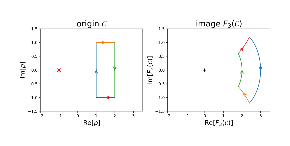
\includegraphics[width=0.9\textwidth]{notebook/fig/output_32_1.eps}
\end{center}
%-------------------------------------------------------------------------------
%-------------------------------------------------------------------------------
\begin{tcolorbox}[breakable, size=fbox, boxrule=1pt, pad at break*=1mm,colback=cellbackground, colframe=cellborder]
\prompt{In}{incolor}{21}{\boxspacing}
\begin{Verbatim}[commandchars=\\\{\}]
\PY{n}{F\PYZus{}3}\PY{o}{.}\PY{n}{cauchy}\PY{p}{(}\PY{n}{C1\PYZus{}inv}\PY{p}{,}\PY{n}{xlim}\PY{o}{=}\PY{p}{(}\PY{o}{\PYZhy{}}\PY{l+m+mi}{2}\PY{p}{,}\PY{l+m+mf}{3.5}\PY{p}{)}\PY{p}{,}\PY{n}{ylim}\PY{o}{=}\PY{p}{(}\PY{o}{\PYZhy{}}\PY{l+m+mf}{1.5}\PY{p}{,}\PY{l+m+mf}{1.5}\PY{p}{)}\PY{p}{,}\PY{n}{contourLabel}\PY{o}{=}\PY{l+s+s2}{\PYZdq{}}\PY{l+s+s2}{C1 (inverse)}\PY{l+s+s2}{\PYZdq{}}\PY{p}{)}
\end{Verbatim}
\end{tcolorbox}
%-------------------------------------------------------------------------------
\begin{center}
    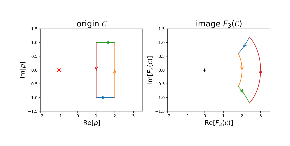
\includegraphics[width=0.9\textwidth]{notebook/fig/output_33_1.eps}
\end{center}
%-------------------------------------------------------------------------------
Nous remarquons tout d'abord que le contour image ne contient pas
l'origine du plan complexe. De plus le contour image est parcouru dans
le même sens que le contour origine. 
%%%%%%%%%%%%%%%%%%%%%%%%%%%%%%%%%%%%%%%%%%%%%%%%%%%%%%%%%%%%%%%%%%%%%%%%%%%%%%%%
\subsubsection{Contour contenant le pôle}
%%%%%%%%%%%%%%%%%%%%%%%%%%%%%%%%%%%%%%%%%%%%%%%%%%%%%%%%%%%%%%%%%%%%%%%%%%%%%%%%
%-------------------------------------------------------------------------------
\begin{tcolorbox}[breakable, size=fbox, boxrule=1pt, pad at break*=1mm,colback=cellbackground, colframe=cellborder]
\prompt{In}{incolor}{22}{\boxspacing}
\begin{Verbatim}[commandchars=\\\{\}]
\PY{n}{F\PYZus{}3}\PY{o}{.}\PY{n}{cauchy}\PY{p}{(}\PY{n}{C2}\PY{p}{,}\PY{n}{xlim}\PY{o}{=}\PY{p}{[}\PY{p}{(}\PY{o}{\PYZhy{}}\PY{l+m+mi}{2}\PY{p}{,}\PY{l+m+mi}{2}\PY{p}{)}\PY{p}{,}\PY{p}{(}\PY{o}{\PYZhy{}}\PY{l+m+mi}{15}\PY{p}{,}\PY{l+m+mi}{15}\PY{p}{)}\PY{p}{]}\PY{p}{,}\PY{n}{ylim}\PY{o}{=}\PY{p}{[}\PY{p}{(}\PY{o}{\PYZhy{}}\PY{l+m+mf}{1.5}\PY{p}{,}\PY{l+m+mf}{1.5}\PY{p}{)}\PY{p}{,}\PY{p}{(}\PY{o}{\PYZhy{}}\PY{l+m+mi}{7}\PY{p}{,}\PY{l+m+mi}{7}\PY{p}{)}\PY{p}{]}\PY{p}{,}\PY{n}{contourLabel}\PY{o}{=}\PY{l+s+s2}{\PYZdq{}}\PY{l+s+s2}{C1}\PY{l+s+s2}{\PYZdq{}}\PY{p}{)}
\end{Verbatim}
\end{tcolorbox}
%-------------------------------------------------------------------------------
%-------------------------------------------------------------------------------
\begin{center}
    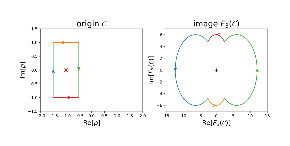
\includegraphics[width=0.9\textwidth]{notebook/fig/output_35_1.eps}
\end{center}
%-------------------------------------------------------------------------------
%-------------------------------------------------------------------------------
\begin{tcolorbox}[breakable, size=fbox, boxrule=1pt, pad at break*=1mm,colback=cellbackground, colframe=cellborder]
\prompt{In}{incolor}{23}{\boxspacing}
\begin{Verbatim}[commandchars=\\\{\}]
\PY{n}{F\PYZus{}3}\PY{o}{.}\PY{n}{cauchy}\PY{p}{(}\PY{n}{C2\PYZus{}inv}\PY{p}{,}\PY{n}{xlim}\PY{o}{=}\PY{p}{[}\PY{p}{(}\PY{o}{\PYZhy{}}\PY{l+m+mi}{2}\PY{p}{,}\PY{l+m+mi}{2}\PY{p}{)}\PY{p}{,}\PY{p}{(}\PY{o}{\PYZhy{}}\PY{l+m+mi}{15}\PY{p}{,}\PY{l+m+mi}{15}\PY{p}{)}\PY{p}{]}\PY{p}{,}\PY{n}{ylim}\PY{o}{=}\PY{p}{[}\PY{p}{(}\PY{o}{\PYZhy{}}\PY{l+m+mf}{1.5}\PY{p}{,}\PY{l+m+mf}{1.5}\PY{p}{)}\PY{p}{,}\PY{p}{(}\PY{o}{\PYZhy{}}\PY{l+m+mi}{7}\PY{p}{,}\PY{l+m+mi}{7}\PY{p}{)}\PY{p}{]}\PY{p}{,}\PY{n}{contourLabel}\PY{o}{=}\PY{l+s+s2}{\PYZdq{}}\PY{l+s+s2}{C1 (inverse)}\PY{l+s+s2}{\PYZdq{}}\PY{p}{)}
\end{Verbatim}
\end{tcolorbox}
%-------------------------------------------------------------------------------
%-------------------------------------------------------------------------------
\begin{center}
    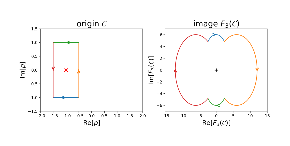
\includegraphics[width=0.9\textwidth]{notebook/fig/output_36_1.eps}
\end{center}
%-------------------------------------------------------------------------------
\textbf{Nous remarquons que l'image du contour entoure l'origine dans le
sens opposé celui du contour d'origine.} Nous allons procédé de la même
manière avec une fonction de transfert possédant deux pôles.
\[
F_4(p)=\dfrac{6}{(p+1)(p+0.75)}
\] 
%%%%%%%%%%%%%%%%%%%%%%%%%%%%%%%%%%%%%%%%%%%%%%%%%%%%%%%%%%%%%%%%%%%%%%%%%%%%%%%%
\subsubsection{Contour ne contenant pas les pôles}
%%%%%%%%%%%%%%%%%%%%%%%%%%%%%%%%%%%%%%%%%%%%%%%%%%%%%%%%%%%%%%%%%%%%%%%%%%%%%%%%
%-------------------------------------------------------------------------------
\begin{tcolorbox}[breakable, size=fbox, boxrule=1pt, pad at break*=1mm,colback=cellbackground, colframe=cellborder]
\prompt{In}{incolor}{24}{\boxspacing}
\begin{Verbatim}[commandchars=\\\{\}]
\PY{n}{zeros}\PY{o}{=}\PY{p}{[}\PY{p}{]}
\PY{n}{poles}\PY{o}{=}\PY{p}{[}\PY{p}{(}\PY{o}{\PYZhy{}}\PY{l+m+mi}{1}\PY{p}{,}\PY{l+m+mi}{0}\PY{p}{)}\PY{p}{,}\PY{p}{(}\PY{o}{\PYZhy{}}\PY{l+m+mf}{0.75}\PY{p}{,}\PY{l+m+mi}{0}\PY{p}{)}\PY{p}{]}
\PY{n}{gain}\PY{o}{=}\PY{l+m+mi}{6}
\PY{n}{F\PYZus{}4}\PY{o}{=}\PY{n}{Ftransfert}\PY{p}{(}\PY{n}{zeros}\PY{o}{=}\PY{n}{zeros}\PY{p}{,}\PY{n}{poles}\PY{o}{=}\PY{n}{poles}\PY{p}{,}\PY{n}{gain}\PY{o}{=}\PY{n}{gain}\PY{p}{,}\PY{n}{name}\PY{o}{=}\PY{l+s+s2}{\PYZdq{}}\PY{l+s+s2}{F\PYZus{}4}\PY{l+s+s2}{\PYZdq{}}\PY{p}{)}
\end{Verbatim}
\end{tcolorbox}
%-------------------------------------------------------------------------------
%-------------------------------------------------------------------------------
\begin{tcolorbox}[breakable, size=fbox, boxrule=1pt, pad at break*=1mm,colback=cellbackground, colframe=cellborder]
\prompt{In}{incolor}{25}{\boxspacing}
\begin{Verbatim}[commandchars=\\\{\}]
\PY{n}{F\PYZus{}4}\PY{o}{.}\PY{n}{cauchy}\PY{p}{(}\PY{n}{C1}\PY{p}{,}\PY{n}{xlim}\PY{o}{=}\PY{p}{(}\PY{o}{\PYZhy{}}\PY{l+m+mi}{2}\PY{p}{,}\PY{l+m+mf}{3.5}\PY{p}{)}\PY{p}{,}\PY{n}{ylim}\PY{o}{=}\PY{p}{(}\PY{o}{\PYZhy{}}\PY{l+m+mf}{1.5}\PY{p}{,}\PY{l+m+mf}{1.5}\PY{p}{)}\PY{p}{,}\PY{n}{contourLabel}\PY{o}{=}\PY{l+s+s2}{\PYZdq{}}\PY{l+s+s2}{C1}\PY{l+s+s2}{\PYZdq{}}\PY{p}{)}
\end{Verbatim}
\end{tcolorbox}
%-------------------------------------------------------------------------------
%-------------------------------------------------------------------------------
\begin{center}
    \includegraphics[width=0.9\textwidth]{notebook/fig/output_39_1.eps}
\end{center}
%-------------------------------------------------------------------------------
%-------------------------------------------------------------------------------
\begin{tcolorbox}[breakable, size=fbox, boxrule=1pt, pad at break*=1mm,colback=cellbackground, colframe=cellborder]
\prompt{In}{incolor}{26}{\boxspacing}
\begin{Verbatim}[commandchars=\\\{\}]
\PY{n}{F\PYZus{}4}\PY{o}{.}\PY{n}{cauchy}\PY{p}{(}\PY{n}{C1\PYZus{}inv}\PY{p}{,}\PY{n}{xlim}\PY{o}{=}\PY{p}{(}\PY{o}{\PYZhy{}}\PY{l+m+mi}{2}\PY{p}{,}\PY{l+m+mf}{3.5}\PY{p}{)}\PY{p}{,}\PY{n}{ylim}\PY{o}{=}\PY{p}{(}\PY{o}{\PYZhy{}}\PY{l+m+mf}{1.5}\PY{p}{,}\PY{l+m+mf}{1.5}\PY{p}{)}\PY{p}{,}\PY{n}{contourLabel}\PY{o}{=}\PY{l+s+s2}{\PYZdq{}}\PY{l+s+s2}{C1 (inverse)}\PY{l+s+s2}{\PYZdq{}}\PY{p}{)}
\end{Verbatim}
\end{tcolorbox}
%-------------------------------------------------------------------------------
%-------------------------------------------------------------------------------
\begin{center}
    \includegraphics[width=0.9\textwidth]{notebook/fig/output_40_1.eps}
\end{center}
%-------------------------------------------------------------------------------
Nous observons comme précédemment que le contour de l'image ne contient pas l'origine. 
%%%%%%%%%%%%%%%%%%%%%%%%%%%%%%%%%%%%%%%%%%%%%%%%%%%%%%%%%%%%%%%%%%%%%%%%%%%%%%%%
\subsubsection{Contour contenant les pôles}
%%%%%%%%%%%%%%%%%%%%%%%%%%%%%%%%%%%%%%%%%%%%%%%%%%%%%%%%%%%%%%%%%%%%%%%%%%%%%%%%
%-------------------------------------------------------------------------------
\begin{tcolorbox}[breakable, size=fbox, boxrule=1pt, pad at break*=1mm,colback=cellbackground, colframe=cellborder]
\prompt{In}{incolor}{27}{\boxspacing}
\begin{Verbatim}[commandchars=\\\{\}]
\PY{n}{F\PYZus{}4}\PY{o}{.}\PY{n}{cauchy}\PY{p}{(}\PY{n}{C3}\PY{p}{,}\PY{n}{xlim}\PY{o}{=}\PY{p}{[}\PY{p}{(}\PY{o}{\PYZhy{}}\PY{l+m+mi}{2}\PY{p}{,}\PY{l+m+mi}{2}\PY{p}{)}\PY{p}{,}\PY{p}{(}\PY{o}{\PYZhy{}}\PY{l+m+mi}{15}\PY{p}{,}\PY{l+m+mi}{20}\PY{p}{)}\PY{p}{]}\PY{p}{,}\PY{n}{ylim}\PY{o}{=}\PY{p}{[}\PY{p}{(}\PY{o}{\PYZhy{}}\PY{l+m+mf}{1.5}\PY{p}{,}\PY{l+m+mf}{1.5}\PY{p}{)}\PY{p}{,}\PY{p}{(}\PY{o}{\PYZhy{}}\PY{l+m+mi}{15}\PY{p}{,}\PY{l+m+mi}{15}\PY{p}{)}\PY{p}{]}\PY{p}{,}\PY{n}{contourLabel}\PY{o}{=}\PY{l+s+s2}{\PYZdq{}}\PY{l+s+s2}{C3}\PY{l+s+s2}{\PYZdq{}}\PY{p}{)}
\end{Verbatim}
\end{tcolorbox}
%-------------------------------------------------------------------------------
%-------------------------------------------------------------------------------
\begin{center}
    
\includegraphics[width=0.9\textwidth]{notebook/fig/output_42_1.eps}
\end{center}
%-------------------------------------------------------------------------------
%-------------------------------------------------------------------------------
\begin{tcolorbox}[breakable, size=fbox, boxrule=1pt, pad at break*=1mm,colback=cellbackground, colframe=cellborder]
\prompt{In}{incolor}{28}{\boxspacing}
\begin{Verbatim}[commandchars=\\\{\}]
\PY{n}{plt}\PY{o}{.}\PY{n}{show}\PY{p}{(}\PY{p}{)}
\PY{n}{F\PYZus{}4}\PY{o}{.}\PY{n}{cauchy}\PY{p}{(}\PY{n}{C3\PYZus{}inv}\PY{p}{,}\PY{n}{xlim}\PY{o}{=}\PY{p}{[}\PY{p}{(}\PY{o}{\PYZhy{}}\PY{l+m+mi}{2}\PY{p}{,}\PY{l+m+mi}{2}\PY{p}{)}\PY{p}{,}\PY{p}{(}\PY{o}{\PYZhy{}}\PY{l+m+mi}{15}\PY{p}{,}\PY{l+m+mi}{20}\PY{p}{)}\PY{p}{]}\PY{p}{,}\PY{n}{ylim}\PY{o}{=}\PY{p}{[}\PY{p}{(}\PY{o}{\PYZhy{}}\PY{l+m+mf}{1.5}\PY{p}{,}\PY{l+m+mf}{1.5}\PY{p}{)}\PY{p}{,}\PY{p}{(}\PY{o}{\PYZhy{}}\PY{l+m+mi}{15}\PY{p}{,}\PY{l+m+mi}{15}\PY{p}{)}\PY{p}{]}\PY{p}{,}\PY{n}{contourLabel}\PY{o}{=}\PY{l+s+s2}{\PYZdq{}}\PY{l+s+s2}{C3 (inverse)}\PY{l+s+s2}{\PYZdq{}}\PY{p}{)}
\end{Verbatim}
\end{tcolorbox}
%-------------------------------------------------------------------------------
%-------------------------------------------------------------------------------
\begin{center}
    
\includegraphics[width=0.9\textwidth]{notebook/fig/output_43_1.eps}
\end{center}
%-------------------------------------------------------------------------------
\textbf{Si le contour entoure un nombre \(P\) de pôles, l'image par la
fonction de transfert de ce contour fait un nombre \(P\) de tours autour
de l'origine dans le sens opposé (à celui du contour).} \# Enoncé du
principe de l'argument de Cauchy On énonce alors le principe de Cauchy:
Si un contour \(\mathcal{C}\) entoure \(Z\) zéros et \(P\) pôles d'une
fonction analytique \(F(p)\) sans en traverser aucun, alors quand on le
parcourt dans le sens anti-trigonométrique, le contour image par
\(F(p)\), \(\Gamma=F(\mathcal{C})\) fait un nombre de tours \(N\) autour
de l'origine dans le sens trigonométrique égal à,
\[
    N=Z-P
\]
On vérifie le principe de Cauchy avec une fonction de transfert composé
de cinq zéros et deux pôles. Et un contour \(\mathcal{C}\) qui contient 
que \(Z=3\) zéros et \(P=1\) pôle. On a donc \(N=2\). Le signe négatif
indique que le nombre de tours est dans le sens opposé au sens
trigonométrique (lorque le contour d'origine tourne dans le sens
horaire.
%-------------------------------------------------------------------------------
\begin{tcolorbox}[breakable, size=fbox, boxrule=1pt, pad at break*=1mm,colback=cellbackground, colframe=cellborder]
\prompt{In}{incolor}{29}{\boxspacing}
\begin{Verbatim}[commandchars=\\\{\}]
\PY{n}{zeros}\PY{o}{=}\PY{p}{[}\PY{p}{(}\PY{o}{\PYZhy{}}\PY{l+m+mf}{0.75}\PY{p}{,}\PY{l+m+mf}{0.5}\PY{p}{)}\PY{p}{,}\PY{p}{(}\PY{o}{\PYZhy{}}\PY{l+m+mf}{0.75}\PY{p}{,}\PY{o}{\PYZhy{}}\PY{l+m+mf}{0.5}\PY{p}{)}\PY{p}{,}\PY{p}{(}\PY{o}{\PYZhy{}}\PY{l+m+mf}{1.65}\PY{p}{,}\PY{l+m+mi}{0}\PY{p}{)}\PY{p}{,}\PY{p}{(}\PY{o}{\PYZhy{}}\PY{l+m+mi}{2}\PY{p}{,}\PY{l+m+mi}{1}\PY{p}{)}\PY{p}{,}\PY{p}{(}\PY{o}{\PYZhy{}}\PY{l+m+mi}{2}\PY{p}{,}\PY{o}{\PYZhy{}}\PY{l+m+mi}{1}\PY{p}{)}\PY{p}{]}
\PY{n}{poles}\PY{o}{=}\PY{p}{[}\PY{p}{(}\PY{o}{\PYZhy{}}\PY{l+m+mi}{1}\PY{p}{,}\PY{l+m+mi}{0}\PY{p}{)}\PY{p}{,}\PY{p}{(}\PY{o}{\PYZhy{}}\PY{l+m+mf}{2.25}\PY{p}{,}\PY{l+m+mi}{0}\PY{p}{)}\PY{p}{]}
\PY{n}{gain}\PY{o}{=}\PY{l+m+mf}{0.75}
\PY{n}{F\PYZus{}5}\PY{o}{=}\PY{n}{Ftransfert}\PY{p}{(}\PY{n}{zeros}\PY{o}{=}\PY{n}{zeros}\PY{p}{,}\PY{n}{poles}\PY{o}{=}\PY{n}{poles}\PY{p}{,}\PY{n}{gain}\PY{o}{=}\PY{n}{gain}\PY{p}{,}\PY{n}{name}\PY{o}{=}\PY{l+s+s2}{\PYZdq{}}\PY{l+s+s2}{F\PYZus{}5}\PY{l+s+s2}{\PYZdq{}}\PY{p}{)}
\PY{n}{F\PYZus{}5}\PY{o}{.}\PY{n}{cauchy}\PY{p}{(}\PY{n}{C3}\PY{p}{,}\PY{n}{xlim}\PY{o}{=}\PY{p}{(}\PY{o}{\PYZhy{}}\PY{l+m+mf}{2.5}\PY{p}{,}\PY{l+m+mf}{1.5}\PY{p}{)}\PY{p}{,}\PY{n}{ylim}\PY{o}{=}\PY{p}{(}\PY{o}{\PYZhy{}}\PY{l+m+mf}{1.5}\PY{p}{,}\PY{l+m+mf}{1.5}\PY{p}{)}\PY{p}{)}
\PY{n}{F\PYZus{}5}\PY{o}{.}\PY{n}{cauchy}\PY{p}{(}\PY{n}{C3\PYZus{}inv}\PY{p}{,}\PY{n}{xlim}\PY{o}{=}\PY{p}{(}\PY{o}{\PYZhy{}}\PY{l+m+mf}{2.5}\PY{p}{,}\PY{l+m+mf}{1.5}\PY{p}{)}\PY{p}{,}\PY{n}{ylim}\PY{o}{=}\PY{p}{(}\PY{o}{\PYZhy{}}\PY{l+m+mf}{1.5}\PY{p}{,}\PY{l+m+mf}{1.5}\PY{p}{)}\PY{p}{)}
\end{Verbatim}
\end{tcolorbox}
%-------------------------------------------------------------------------------
%-------------------------------------------------------------------------------
\begin{center}
    
\includegraphics[width=0.9\textwidth]{notebook/fig/output_45_1.eps}
\end{center}
%-------------------------------------------------------------------------------
%-------------------------------------------------------------------------------
\begin{center}
    
\includegraphics[width=0.9\textwidth]{notebook/fig/output_45_2.eps}
\end{center}
%-------------------------------------------------------------------------------
